\section{Durchführung}
\label{sec:Durchführung}

\subsection{Aufbau}

Der schematische Versuchsaufbau ist in Abbildung \ref{fig:aufbau1} dargestellt. Die einzelnen Bauteile und deren Funktion werden im Folgenden genauer beschrieben. Die 
Funktionsweise des Szintillators wurde bereits im Kontext des Abschnittes \ref{sec:Theorie} beeschrieben, weshalb hier nicht genauer darauf eingegangen wird.

\begin{figure}
    \centering
    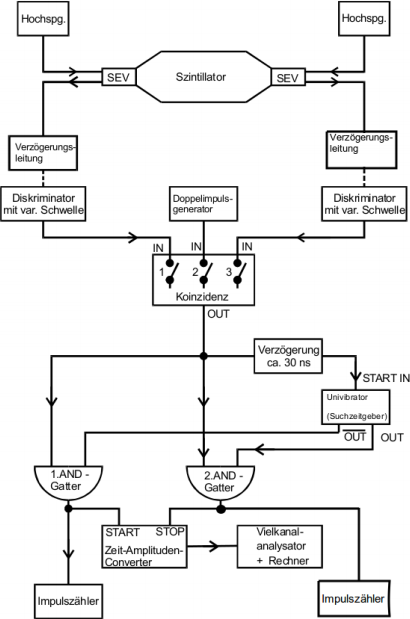
\includegraphics[width=\textwidth]{data/aufbau_skizze_1.png}
    \caption{Schematischer Aufbau des Versuchs}
    \label{fig:aufbau1}
\end{figure}

Die Signale, welche vom Szintillator an die Photomultiplier (PMT) weitergeleitet werden, sind durch Energieniveauübergänge entstehende Photonen. Diese treffen zuerst auf eine Photokathode,
wodurch ein Elektron emittiert wird, welches dann auf mehrere hintereinander geschaltete Elektroden unter Hochspannung trifft und somit Sekundärelektronen auslöst, um einen messbaren
Ladungsimpuls zu erzeugen. Es kann nicht davon ausgegangen werden, dass die beiden Photomultiplier die exakt gleiche Ansprechzeit haben, weshalb dies über eine Verzögerungsleitung 
angepasst wird. Noch vor der Verzögerungsleitung wird außerdem auf beiden Seiten jeweils ein Diskriminator eingebaut, der dafür sorgt, dass ein Untergrundrauschen unterdrückt wird.
Die auf diese Weise modifizierten Signale treffen dann von beiden Seiten auf eine Koinzidenzschaltung, die nur dann ein Signal weitergibt, wenn es von beiden Seiten gleichzeitig,
bzw. innerhalb eines Zeitintervalls $\Delta t_\text{K} $ ankommt. 
Danach folgen in der Schaltung zwei AND-Gatter, die im Zusammenspiel mit einem Monoflop dazu dienen, ein Startsignal von einem Stoppsignal unterscheiden zu können. beide AND-Gatter
sind sowohl direkt mit der Koinzidenz, als auch an den Monoflop, der wiederum über eine $\SI{30}{ns}$ Verzögerungsleitung mit der Koinzidenz verbunden ist. Wird ein Signal von einem 
der beiden AND-Gatter registriert, wird dieses als Startsignal gewertet und[] lang ein Suchfenster geöffnet. Wird während dieser Zeit ein weiteres Signal registriert, so wird dieses 
als Stoppsignal gewertet, was den Zerfall des mit dem Startsignal eingetroffenen Myons mitteilt. Wird innerhalb des Suchfensters kein weiteres Signal detektiert, wird das nächste Signal 
wieder als Startsignal gewertet. Beide AND-Gatter sind außerdem mit 
dem dahinter befindlichen Time-Amplitude-Converter (TAC) verbunden, der die Dauer zwischen einem Startsignal und einem Stoppsignal misst, um diese in eine Spannung zu 
übersetzen. Von da aus werden die Signale weiter an den Multi-Channel-Analyzer (MAC) und den zur Auswertung der Messwerte notwendigen PC gegeben.
% Mit diesem Aufbau kann gewährleistet werden, dass ein Signal eines eintreffeden Myons von dem eines Zerfalls unterschieden wird, um somit die individuellen Lebensdauern der Myonen messen zu können. 

\subsection{Kalibrierung}

Bevor die eigentlich Messung beginnen kann, müssen einige Komponenten justiert werden. Dafür werden zuerst die beiden PMTs an die Diskriminatoren, und diese wiederum an einen 
Oszillographen angeschlossen. Damit sollten von beiden PMTs Impulse in Form von Auslenkungen auf dem Oszillographen sichtbar sein, welche jeweils gleich stark sein müssen. 
Bei einer Abweichung der Intensität der Impulse der unterschiedlichen PMTs wird an den Diskriminatoren nachjustiert, bis durch beide PMTs die gleiche Intensität der Auslenkungen
auf dem Oszillographen zu sehen ist. Danach wird die Koinzidenz mitsam Verzögerungsleitung angeschlossen. Unter Variation der Verzögerungen wird das Signal der Koinzidenz auf ein Zählwerk 
weitergeleitet, wobei die Zählrate gegen die relative Verzögerung aufgetragen wird, sodass ein Maximum, welches als Plateau auftritt, bestimmt werden kann. Optimalerweise sollte 
sich die Verzögerung in der Mitte des Plateaus befinden. Um die richtige Schwelle der Diskriminatoren zu überprüfen, werden die Zählraten vor und nach diesem verglichen. Weichen 
die beiden Zählraten nicht oder kaum voneinander ab, so wird die Schwelle des Diskriminators gesenkt, damit keine Signale abgefangen werden, die gemessen werden sollen. \\
Nun wird der eben genannte Aufbau von der restlichen Schaltung getrennt und anstelle dessen ein Doppelimpulsgenerator angeschlossen. Nachdem die Verzögerung und der 
Univibrator(Suchzeitgeber) angeschlossen werden, kann nun der TAC auf eine Suchzeit $t_\text{s}$ eigestellt werden. Die daraufhin angeschlossen AND-Gatter werden dann mit dem 
Oszillographen getestet, wobei die Zeitintervalle der im TAC eintreffeden Signale überprüft werden. Die Zeitabstände der Doppelimpulse können dann variiert werden, wodurch den 
Kanälen des MAC jeweils eine Zeitdauer zugeordnet werden kann. Damit ist die Justage des Versuchs vollendet und der Anfangs beschriebene Teil kann wieder anstelle des Doppelimpulsgenerator
angeschlossen werden, um die Messung zu starten.